% backtracking worksheet template
\documentclass[leqno, 12pt]{article}
\usepackage{tikz} 
\usetikzlibrary{positioning}
\usetikzlibrary {arrows.meta}
\usepackage[a4paper, portrait, margin=1cm]{geometry}
\usepackage{multicol}
\pagestyle{empty}

\tikzset{backtrack/.style={rectangle,draw=black,fill=white,
inner sep=2pt,minimum height=32pt, minimum width=20mm}}
\tikzset{backtrackeq/.style={rectangle,draw=black,fill=white,
inner sep=2pt,minimum height=12pt, minimum width=20mm}}
\tikzset{backtrackstep/.style={rectangle,draw=none,fill=white,
inner sep=2pt,minimum height=12pt, minimum width=20mm}}

\def \HeadingAnswers {\section*{\Large Name: \underline{\hspace{8cm}} \hfill Date: \underline{\hspace{3cm}}} \vspace{-3mm}
{2-step backtracking: Answers} \vspace{1pt}\hrule}

\begin{document}
    \HeadingAnswers
    \vspace{-8mm}
    \begin{multicols}{2}
        \begin{equation}
    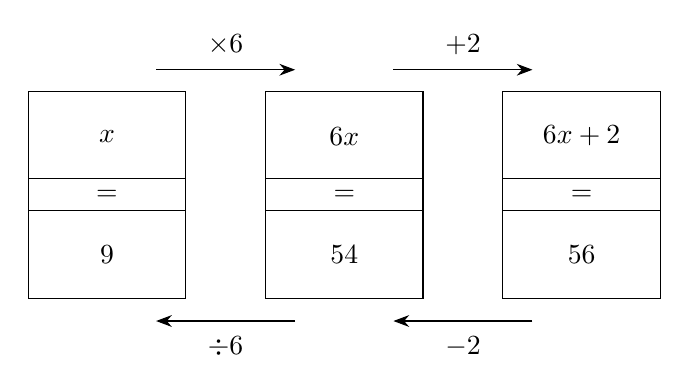
\begin{tikzpicture}[baseline={([yshift=-12pt]current bounding box.north)}]
            
        \node[backtrack] (boxA) at (0, 0) {$x$};
        \node[backtrack] (boxB) [right=1cm of boxA] {$6x$};
        \node[backtrack] (boxC) [right=1cm of boxB] {$6x + 2$};
    
        \node[backtrackeq] (boxAeq) [below=-1pt of boxA] {$=$};
        \node[backtrackeq] (boxBeq) [below=-1pt of boxB] {$=$};
        \node[backtrackeq] (boxCeq) [below=-1pt of boxC] {$=$};
        
        \node[backtrack] (boxArev) [below=-1pt of boxAeq] {$9$};
        \node[backtrack] (boxBrev) [below=-1pt of boxBeq] {$54$};
        \node[backtrack] (boxCrev) [below=-1pt of boxCeq] {$56$};
         
        \node (boxAr) at ([yshift=24pt,xshift=5mm]boxA) { };
        \node (boxBl) at ([yshift=24pt,xshift=-5mm]boxB) { };
        \draw [line width=0.4pt,-{Stealth[length=2mm]}] (boxAr)  --node[backtrackstep, above=3.0pt] {$\times6$} (boxBl);
    
        \node (boxBr) at ([yshift=24pt,xshift=5mm]boxB) { };
        \node (boxCl) at ([yshift=24pt,xshift=-5mm]boxC) { };
        \draw [line width=0.4pt,-{Stealth[length=2mm]}] (boxBr)  --node[backtrackstep, above=3.0pt] {$+2$} (boxCl);
    
        \node (boxCrevl) at ([yshift=-24pt,xshift=-5mm]boxCrev) { };
        \node (boxBrevr) at ([yshift=-24pt,xshift=5mm]boxBrev) { };
        \draw [line width=0.4pt,-{Stealth[length=2mm]}] (boxCrevl)  --node[backtrackstep, below=3.0pt] {$-2$} (boxBrevr);
    
        \node (boxBrevl) at ([yshift=-24pt,xshift=-5mm]boxBrev) { };
        \node (boxArevr) at ([yshift=-24pt,xshift=5mm]boxArev) { };
        \draw [line width=0.4pt,-{Stealth[length=2mm]}] (boxBrevl)  --node[backtrackstep, below=3.0pt] {$\div6$} (boxArevr);
        
    \end{tikzpicture}    
\end{equation}


\vspace{-2pt}\begin{equation}
    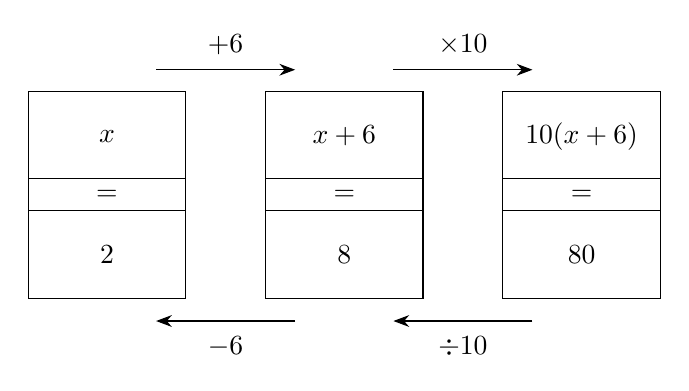
\begin{tikzpicture}[baseline={([yshift=-12pt]current bounding box.north)}]
            
        \node[backtrack] (boxA) at (0, 0) {$x$};
        \node[backtrack] (boxB) [right=1cm of boxA] {$x+6$};
        \node[backtrack] (boxC) [right=1cm of boxB] {$10(x + 6)$};
    
        \node[backtrackeq] (boxAeq) [below=-1pt of boxA] {$=$};
        \node[backtrackeq] (boxBeq) [below=-1pt of boxB] {$=$};
        \node[backtrackeq] (boxCeq) [below=-1pt of boxC] {$=$};
        
        \node[backtrack] (boxArev) [below=-1pt of boxAeq] {$2$};
        \node[backtrack] (boxBrev) [below=-1pt of boxBeq] {$8$};
        \node[backtrack] (boxCrev) [below=-1pt of boxCeq] {$80$};
         
        \node (boxAr) at ([yshift=24pt,xshift=5mm]boxA) { };
        \node (boxBl) at ([yshift=24pt,xshift=-5mm]boxB) { };
        \draw [line width=0.4pt,-{Stealth[length=2mm]}] (boxAr)  --node[backtrackstep, above=3.0pt] {$+6$} (boxBl);
    
        \node (boxBr) at ([yshift=24pt,xshift=5mm]boxB) { };
        \node (boxCl) at ([yshift=24pt,xshift=-5mm]boxC) { };
        \draw [line width=0.4pt,-{Stealth[length=2mm]}] (boxBr)  --node[backtrackstep, above=3.0pt] {$\times10$} (boxCl);
    
        \node (boxCrevl) at ([yshift=-24pt,xshift=-5mm]boxCrev) { };
        \node (boxBrevr) at ([yshift=-24pt,xshift=5mm]boxBrev) { };
        \draw [line width=0.4pt,-{Stealth[length=2mm]}] (boxCrevl)  --node[backtrackstep, below=3.0pt] {$\div10$} (boxBrevr);
    
        \node (boxBrevl) at ([yshift=-24pt,xshift=-5mm]boxBrev) { };
        \node (boxArevr) at ([yshift=-24pt,xshift=5mm]boxArev) { };
        \draw [line width=0.4pt,-{Stealth[length=2mm]}] (boxBrevl)  --node[backtrackstep, below=3.0pt] {$-6$} (boxArevr);
        
    \end{tikzpicture}    
\end{equation}


\vspace{-2pt}\begin{equation}
    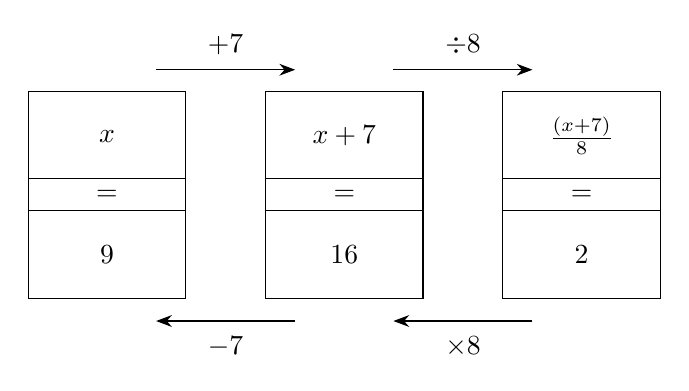
\begin{tikzpicture}[baseline={([yshift=-12pt]current bounding box.north)}]
            
        \node[backtrack] (boxA) at (0, 0) {$x$};
        \node[backtrack] (boxB) [right=1cm of boxA] {$x+7$};
        \node[backtrack] (boxC) [right=1cm of boxB] {$\frac{(x+7)}{8}$};
    
        \node[backtrackeq] (boxAeq) [below=-1pt of boxA] {$=$};
        \node[backtrackeq] (boxBeq) [below=-1pt of boxB] {$=$};
        \node[backtrackeq] (boxCeq) [below=-1pt of boxC] {$=$};
        
        \node[backtrack] (boxArev) [below=-1pt of boxAeq] {$9$};
        \node[backtrack] (boxBrev) [below=-1pt of boxBeq] {$16$};
        \node[backtrack] (boxCrev) [below=-1pt of boxCeq] {$2$};
         
        \node (boxAr) at ([yshift=24pt,xshift=5mm]boxA) { };
        \node (boxBl) at ([yshift=24pt,xshift=-5mm]boxB) { };
        \draw [line width=0.4pt,-{Stealth[length=2mm]}] (boxAr)  --node[backtrackstep, above=3.0pt] {$+7$} (boxBl);
    
        \node (boxBr) at ([yshift=24pt,xshift=5mm]boxB) { };
        \node (boxCl) at ([yshift=24pt,xshift=-5mm]boxC) { };
        \draw [line width=0.4pt,-{Stealth[length=2mm]}] (boxBr)  --node[backtrackstep, above=3.0pt] {$\div8$} (boxCl);
    
        \node (boxCrevl) at ([yshift=-24pt,xshift=-5mm]boxCrev) { };
        \node (boxBrevr) at ([yshift=-24pt,xshift=5mm]boxBrev) { };
        \draw [line width=0.4pt,-{Stealth[length=2mm]}] (boxCrevl)  --node[backtrackstep, below=3.0pt] {$\times8$} (boxBrevr);
    
        \node (boxBrevl) at ([yshift=-24pt,xshift=-5mm]boxBrev) { };
        \node (boxArevr) at ([yshift=-24pt,xshift=5mm]boxArev) { };
        \draw [line width=0.4pt,-{Stealth[length=2mm]}] (boxBrevl)  --node[backtrackstep, below=3.0pt] {$-7$} (boxArevr);
        
    \end{tikzpicture}    
\end{equation}


\vspace{-2pt}\begin{equation}
    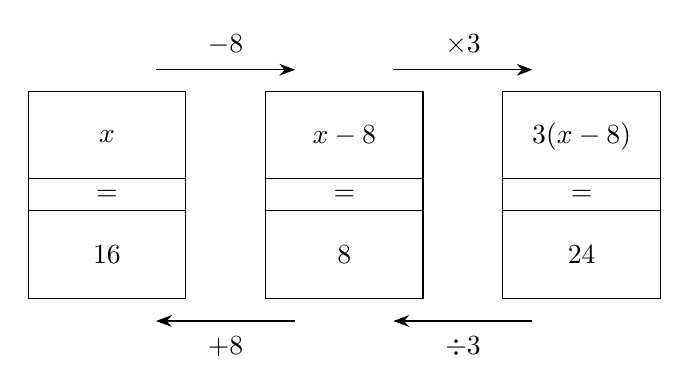
\begin{tikzpicture}[baseline={([yshift=-12pt]current bounding box.north)}]
            
        \node[backtrack] (boxA) at (0, 0) {$x$};
        \node[backtrack] (boxB) [right=1cm of boxA] {$x-8$};
        \node[backtrack] (boxC) [right=1cm of boxB] {$3(x-8)$};
    
        \node[backtrackeq] (boxAeq) [below=-1pt of boxA] {$=$};
        \node[backtrackeq] (boxBeq) [below=-1pt of boxB] {$=$};
        \node[backtrackeq] (boxCeq) [below=-1pt of boxC] {$=$};
        
        \node[backtrack] (boxArev) [below=-1pt of boxAeq] {$16$};
        \node[backtrack] (boxBrev) [below=-1pt of boxBeq] {$8$};
        \node[backtrack] (boxCrev) [below=-1pt of boxCeq] {$24$};
         
        \node (boxAr) at ([yshift=24pt,xshift=5mm]boxA) { };
        \node (boxBl) at ([yshift=24pt,xshift=-5mm]boxB) { };
        \draw [line width=0.4pt,-{Stealth[length=2mm]}] (boxAr)  --node[backtrackstep, above=3.0pt] {$-8$} (boxBl);
    
        \node (boxBr) at ([yshift=24pt,xshift=5mm]boxB) { };
        \node (boxCl) at ([yshift=24pt,xshift=-5mm]boxC) { };
        \draw [line width=0.4pt,-{Stealth[length=2mm]}] (boxBr)  --node[backtrackstep, above=3.0pt] {$\times3$} (boxCl);
    
        \node (boxCrevl) at ([yshift=-24pt,xshift=-5mm]boxCrev) { };
        \node (boxBrevr) at ([yshift=-24pt,xshift=5mm]boxBrev) { };
        \draw [line width=0.4pt,-{Stealth[length=2mm]}] (boxCrevl)  --node[backtrackstep, below=3.0pt] {$\div3$} (boxBrevr);
    
        \node (boxBrevl) at ([yshift=-24pt,xshift=-5mm]boxBrev) { };
        \node (boxArevr) at ([yshift=-24pt,xshift=5mm]boxArev) { };
        \draw [line width=0.4pt,-{Stealth[length=2mm]}] (boxBrevl)  --node[backtrackstep, below=3.0pt] {$+8$} (boxArevr);
        
    \end{tikzpicture}    
\end{equation}


\vspace{-2pt}\begin{equation}
    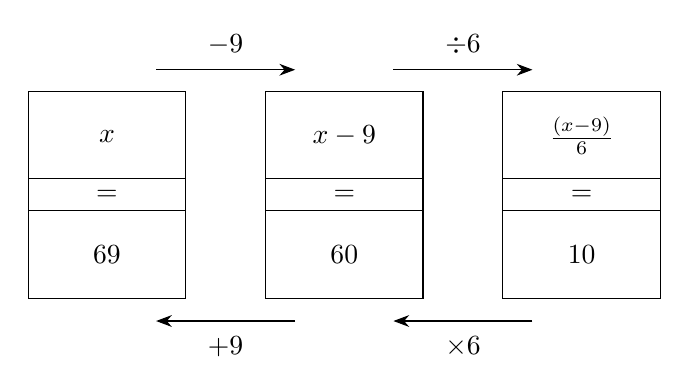
\begin{tikzpicture}[baseline={([yshift=-12pt]current bounding box.north)}]
            
        \node[backtrack] (boxA) at (0, 0) {$x$};
        \node[backtrack] (boxB) [right=1cm of boxA] {$x-9$};
        \node[backtrack] (boxC) [right=1cm of boxB] {$\frac{(x-9)}{6}$};
    
        \node[backtrackeq] (boxAeq) [below=-1pt of boxA] {$=$};
        \node[backtrackeq] (boxBeq) [below=-1pt of boxB] {$=$};
        \node[backtrackeq] (boxCeq) [below=-1pt of boxC] {$=$};
        
        \node[backtrack] (boxArev) [below=-1pt of boxAeq] {$69$};
        \node[backtrack] (boxBrev) [below=-1pt of boxBeq] {$60$};
        \node[backtrack] (boxCrev) [below=-1pt of boxCeq] {$10$};
         
        \node (boxAr) at ([yshift=24pt,xshift=5mm]boxA) { };
        \node (boxBl) at ([yshift=24pt,xshift=-5mm]boxB) { };
        \draw [line width=0.4pt,-{Stealth[length=2mm]}] (boxAr)  --node[backtrackstep, above=3.0pt] {$-9$} (boxBl);
    
        \node (boxBr) at ([yshift=24pt,xshift=5mm]boxB) { };
        \node (boxCl) at ([yshift=24pt,xshift=-5mm]boxC) { };
        \draw [line width=0.4pt,-{Stealth[length=2mm]}] (boxBr)  --node[backtrackstep, above=3.0pt] {$\div6$} (boxCl);
    
        \node (boxCrevl) at ([yshift=-24pt,xshift=-5mm]boxCrev) { };
        \node (boxBrevr) at ([yshift=-24pt,xshift=5mm]boxBrev) { };
        \draw [line width=0.4pt,-{Stealth[length=2mm]}] (boxCrevl)  --node[backtrackstep, below=3.0pt] {$\times6$} (boxBrevr);
    
        \node (boxBrevl) at ([yshift=-24pt,xshift=-5mm]boxBrev) { };
        \node (boxArevr) at ([yshift=-24pt,xshift=5mm]boxArev) { };
        \draw [line width=0.4pt,-{Stealth[length=2mm]}] (boxBrevl)  --node[backtrackstep, below=3.0pt] {$+9$} (boxArevr);
        
    \end{tikzpicture}    
\end{equation}


\vspace{-2pt}
    \columnbreak
        \begin{equation}
    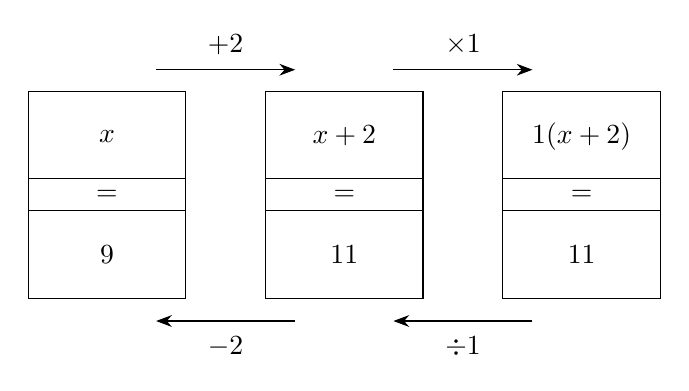
\begin{tikzpicture}[baseline={([yshift=-12pt]current bounding box.north)}]
            
        \node[backtrack] (boxA) at (0, 0) {$x$};
        \node[backtrack] (boxB) [right=1cm of boxA] {$x+2$};
        \node[backtrack] (boxC) [right=1cm of boxB] {$1(x + 2)$};
    
        \node[backtrackeq] (boxAeq) [below=-1pt of boxA] {$=$};
        \node[backtrackeq] (boxBeq) [below=-1pt of boxB] {$=$};
        \node[backtrackeq] (boxCeq) [below=-1pt of boxC] {$=$};
        
        \node[backtrack] (boxArev) [below=-1pt of boxAeq] {$9$};
        \node[backtrack] (boxBrev) [below=-1pt of boxBeq] {$11$};
        \node[backtrack] (boxCrev) [below=-1pt of boxCeq] {$11$};
         
        \node (boxAr) at ([yshift=24pt,xshift=5mm]boxA) { };
        \node (boxBl) at ([yshift=24pt,xshift=-5mm]boxB) { };
        \draw [line width=0.4pt,-{Stealth[length=2mm]}] (boxAr)  --node[backtrackstep, above=3.0pt] {$+2$} (boxBl);
    
        \node (boxBr) at ([yshift=24pt,xshift=5mm]boxB) { };
        \node (boxCl) at ([yshift=24pt,xshift=-5mm]boxC) { };
        \draw [line width=0.4pt,-{Stealth[length=2mm]}] (boxBr)  --node[backtrackstep, above=3.0pt] {$\times1$} (boxCl);
    
        \node (boxCrevl) at ([yshift=-24pt,xshift=-5mm]boxCrev) { };
        \node (boxBrevr) at ([yshift=-24pt,xshift=5mm]boxBrev) { };
        \draw [line width=0.4pt,-{Stealth[length=2mm]}] (boxCrevl)  --node[backtrackstep, below=3.0pt] {$\div1$} (boxBrevr);
    
        \node (boxBrevl) at ([yshift=-24pt,xshift=-5mm]boxBrev) { };
        \node (boxArevr) at ([yshift=-24pt,xshift=5mm]boxArev) { };
        \draw [line width=0.4pt,-{Stealth[length=2mm]}] (boxBrevl)  --node[backtrackstep, below=3.0pt] {$-2$} (boxArevr);
        
    \end{tikzpicture}    
\end{equation}


\vspace{-2pt}\begin{equation}
    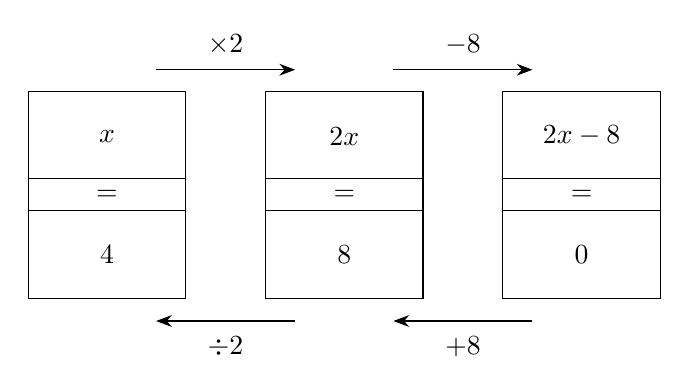
\begin{tikzpicture}[baseline={([yshift=-12pt]current bounding box.north)}]
            
        \node[backtrack] (boxA) at (0, 0) {$x$};
        \node[backtrack] (boxB) [right=1cm of boxA] {$2x$};
        \node[backtrack] (boxC) [right=1cm of boxB] {$2x - 8$};
    
        \node[backtrackeq] (boxAeq) [below=-1pt of boxA] {$=$};
        \node[backtrackeq] (boxBeq) [below=-1pt of boxB] {$=$};
        \node[backtrackeq] (boxCeq) [below=-1pt of boxC] {$=$};
        
        \node[backtrack] (boxArev) [below=-1pt of boxAeq] {$4$};
        \node[backtrack] (boxBrev) [below=-1pt of boxBeq] {$8$};
        \node[backtrack] (boxCrev) [below=-1pt of boxCeq] {$0$};
         
        \node (boxAr) at ([yshift=24pt,xshift=5mm]boxA) { };
        \node (boxBl) at ([yshift=24pt,xshift=-5mm]boxB) { };
        \draw [line width=0.4pt,-{Stealth[length=2mm]}] (boxAr)  --node[backtrackstep, above=3.0pt] {$\times2$} (boxBl);
    
        \node (boxBr) at ([yshift=24pt,xshift=5mm]boxB) { };
        \node (boxCl) at ([yshift=24pt,xshift=-5mm]boxC) { };
        \draw [line width=0.4pt,-{Stealth[length=2mm]}] (boxBr)  --node[backtrackstep, above=3.0pt] {$-8$} (boxCl);
    
        \node (boxCrevl) at ([yshift=-24pt,xshift=-5mm]boxCrev) { };
        \node (boxBrevr) at ([yshift=-24pt,xshift=5mm]boxBrev) { };
        \draw [line width=0.4pt,-{Stealth[length=2mm]}] (boxCrevl)  --node[backtrackstep, below=3.0pt] {$+8$} (boxBrevr);
    
        \node (boxBrevl) at ([yshift=-24pt,xshift=-5mm]boxBrev) { };
        \node (boxArevr) at ([yshift=-24pt,xshift=5mm]boxArev) { };
        \draw [line width=0.4pt,-{Stealth[length=2mm]}] (boxBrevl)  --node[backtrackstep, below=3.0pt] {$\div2$} (boxArevr);
        
    \end{tikzpicture}    
\end{equation}


\vspace{-2pt}\begin{equation}
    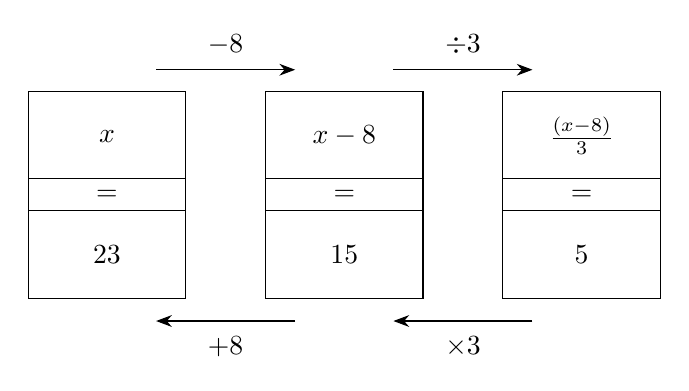
\begin{tikzpicture}[baseline={([yshift=-12pt]current bounding box.north)}]
            
        \node[backtrack] (boxA) at (0, 0) {$x$};
        \node[backtrack] (boxB) [right=1cm of boxA] {$x-8$};
        \node[backtrack] (boxC) [right=1cm of boxB] {$\frac{(x-8)}{3}$};
    
        \node[backtrackeq] (boxAeq) [below=-1pt of boxA] {$=$};
        \node[backtrackeq] (boxBeq) [below=-1pt of boxB] {$=$};
        \node[backtrackeq] (boxCeq) [below=-1pt of boxC] {$=$};
        
        \node[backtrack] (boxArev) [below=-1pt of boxAeq] {$23$};
        \node[backtrack] (boxBrev) [below=-1pt of boxBeq] {$15$};
        \node[backtrack] (boxCrev) [below=-1pt of boxCeq] {$5$};
         
        \node (boxAr) at ([yshift=24pt,xshift=5mm]boxA) { };
        \node (boxBl) at ([yshift=24pt,xshift=-5mm]boxB) { };
        \draw [line width=0.4pt,-{Stealth[length=2mm]}] (boxAr)  --node[backtrackstep, above=3.0pt] {$-8$} (boxBl);
    
        \node (boxBr) at ([yshift=24pt,xshift=5mm]boxB) { };
        \node (boxCl) at ([yshift=24pt,xshift=-5mm]boxC) { };
        \draw [line width=0.4pt,-{Stealth[length=2mm]}] (boxBr)  --node[backtrackstep, above=3.0pt] {$\div3$} (boxCl);
    
        \node (boxCrevl) at ([yshift=-24pt,xshift=-5mm]boxCrev) { };
        \node (boxBrevr) at ([yshift=-24pt,xshift=5mm]boxBrev) { };
        \draw [line width=0.4pt,-{Stealth[length=2mm]}] (boxCrevl)  --node[backtrackstep, below=3.0pt] {$\times3$} (boxBrevr);
    
        \node (boxBrevl) at ([yshift=-24pt,xshift=-5mm]boxBrev) { };
        \node (boxArevr) at ([yshift=-24pt,xshift=5mm]boxArev) { };
        \draw [line width=0.4pt,-{Stealth[length=2mm]}] (boxBrevl)  --node[backtrackstep, below=3.0pt] {$+8$} (boxArevr);
        
    \end{tikzpicture}    
\end{equation}


\vspace{-2pt}\begin{equation}
    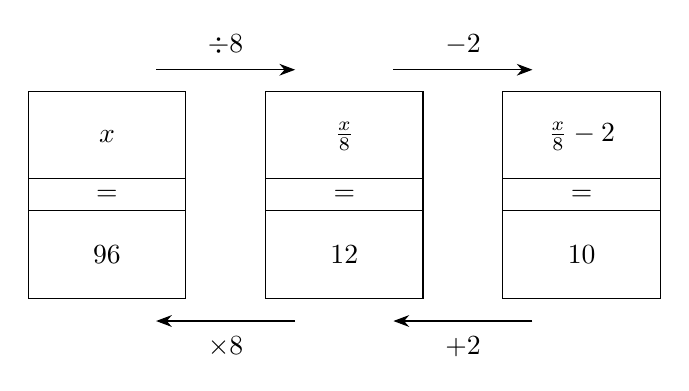
\begin{tikzpicture}[baseline={([yshift=-12pt]current bounding box.north)}]
            
        \node[backtrack] (boxA) at (0, 0) {$x$};
        \node[backtrack] (boxB) [right=1cm of boxA] {$\frac{x}{8}$};
        \node[backtrack] (boxC) [right=1cm of boxB] {$\frac{x}{8} - 2$};
    
        \node[backtrackeq] (boxAeq) [below=-1pt of boxA] {$=$};
        \node[backtrackeq] (boxBeq) [below=-1pt of boxB] {$=$};
        \node[backtrackeq] (boxCeq) [below=-1pt of boxC] {$=$};
        
        \node[backtrack] (boxArev) [below=-1pt of boxAeq] {$96$};
        \node[backtrack] (boxBrev) [below=-1pt of boxBeq] {$12$};
        \node[backtrack] (boxCrev) [below=-1pt of boxCeq] {$10$};
         
        \node (boxAr) at ([yshift=24pt,xshift=5mm]boxA) { };
        \node (boxBl) at ([yshift=24pt,xshift=-5mm]boxB) { };
        \draw [line width=0.4pt,-{Stealth[length=2mm]}] (boxAr)  --node[backtrackstep, above=3.0pt] {$\div8$} (boxBl);
    
        \node (boxBr) at ([yshift=24pt,xshift=5mm]boxB) { };
        \node (boxCl) at ([yshift=24pt,xshift=-5mm]boxC) { };
        \draw [line width=0.4pt,-{Stealth[length=2mm]}] (boxBr)  --node[backtrackstep, above=3.0pt] {$-2$} (boxCl);
    
        \node (boxCrevl) at ([yshift=-24pt,xshift=-5mm]boxCrev) { };
        \node (boxBrevr) at ([yshift=-24pt,xshift=5mm]boxBrev) { };
        \draw [line width=0.4pt,-{Stealth[length=2mm]}] (boxCrevl)  --node[backtrackstep, below=3.0pt] {$+2$} (boxBrevr);
    
        \node (boxBrevl) at ([yshift=-24pt,xshift=-5mm]boxBrev) { };
        \node (boxArevr) at ([yshift=-24pt,xshift=5mm]boxArev) { };
        \draw [line width=0.4pt,-{Stealth[length=2mm]}] (boxBrevl)  --node[backtrackstep, below=3.0pt] {$\times8$} (boxArevr);
        
    \end{tikzpicture}    
\end{equation}


\vspace{-2pt}\begin{equation}
    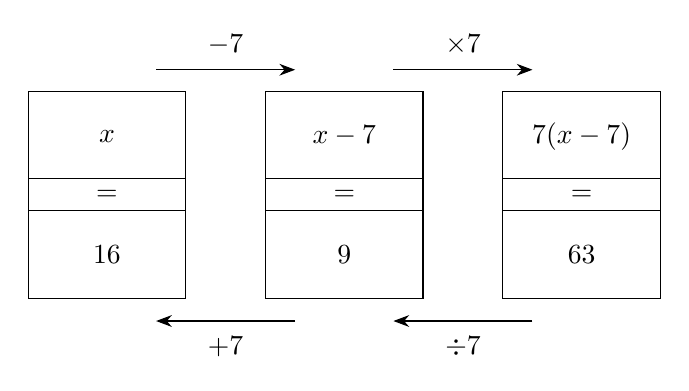
\begin{tikzpicture}[baseline={([yshift=-12pt]current bounding box.north)}]
            
        \node[backtrack] (boxA) at (0, 0) {$x$};
        \node[backtrack] (boxB) [right=1cm of boxA] {$x-7$};
        \node[backtrack] (boxC) [right=1cm of boxB] {$7(x-7)$};
    
        \node[backtrackeq] (boxAeq) [below=-1pt of boxA] {$=$};
        \node[backtrackeq] (boxBeq) [below=-1pt of boxB] {$=$};
        \node[backtrackeq] (boxCeq) [below=-1pt of boxC] {$=$};
        
        \node[backtrack] (boxArev) [below=-1pt of boxAeq] {$16$};
        \node[backtrack] (boxBrev) [below=-1pt of boxBeq] {$9$};
        \node[backtrack] (boxCrev) [below=-1pt of boxCeq] {$63$};
         
        \node (boxAr) at ([yshift=24pt,xshift=5mm]boxA) { };
        \node (boxBl) at ([yshift=24pt,xshift=-5mm]boxB) { };
        \draw [line width=0.4pt,-{Stealth[length=2mm]}] (boxAr)  --node[backtrackstep, above=3.0pt] {$-7$} (boxBl);
    
        \node (boxBr) at ([yshift=24pt,xshift=5mm]boxB) { };
        \node (boxCl) at ([yshift=24pt,xshift=-5mm]boxC) { };
        \draw [line width=0.4pt,-{Stealth[length=2mm]}] (boxBr)  --node[backtrackstep, above=3.0pt] {$\times7$} (boxCl);
    
        \node (boxCrevl) at ([yshift=-24pt,xshift=-5mm]boxCrev) { };
        \node (boxBrevr) at ([yshift=-24pt,xshift=5mm]boxBrev) { };
        \draw [line width=0.4pt,-{Stealth[length=2mm]}] (boxCrevl)  --node[backtrackstep, below=3.0pt] {$\div7$} (boxBrevr);
    
        \node (boxBrevl) at ([yshift=-24pt,xshift=-5mm]boxBrev) { };
        \node (boxArevr) at ([yshift=-24pt,xshift=5mm]boxArev) { };
        \draw [line width=0.4pt,-{Stealth[length=2mm]}] (boxBrevl)  --node[backtrackstep, below=3.0pt] {$+7$} (boxArevr);
        
    \end{tikzpicture}    
\end{equation}


\vspace{-2pt}
    \end{multicols}
\end{document}
